
\chapter{Special Elements} \label{SpecElem}

One advantage of SixTrack, that has been adopted from RACETRACK, is that it easily allows to define elements for a specific purpose. The special elements implemented till now are found in this section.
All Special Elements should be written in the \texttt{fort.3} file.

% ================================================================================================================================ %
\section{Multipole Coefficients} \label{MulCoe}

Sets of normal and skew multipoles of up to tenth order, each with an r.m.s. value, can be combined with this block.
The multipole kick is calculated using a Horner scheme, which saves considerably in computation time.
Moreover, using the multipole block reduces the number of elements in the single element list (\ref{SinEle}).

\bigskip
\begin{tabular}{@{}lp{0.8\linewidth}}
    \textbf{Keyword}    & \texttt{MULT} \\
    \textbf{Data lines} & 2 to 12 \\
    \textbf{Format}     & First line: \texttt{name $R_{0}$ $\delta_{0}$} \\
                        & Lines 2 to 12: \texttt{$B_{n}$ rms-$B_{n}$ $A_{n}$ rms-$A_{n}$}
\end{tabular}

\paragraph{Format Description}~

\bigskip
\begin{tabular}{@{}lp{0.8\linewidth}}
    \texttt{name}    & Name of the multipole block which must appear in the list of single elements (\ref{MulBlo}). \\
    \texttt{$R_{0}$} & Reference radius (in mm) at which the magnet errors are calculated. This makes it convenient to use values from field measurements. \\
    \texttt{$\delta_{0}$} & Bending strength of the dipole (in mrad). Field errors of line 2--11 are taken to be relative to the bending strength.
\end{tabular}

\paragraph{Remarks:}
\begin{enumerate}
    \item The $B_{n}$ and $A_{n}$ are related to the $b_{n}, a_{n}$ of the single nonlinear element (\ref{NonEle}) in the following way:
        \begin{align*}
            b_{n} &= \delta_{0} B_{n} R_{0}^{1-n} 10^{3n-6} \\
            a_{n} &= \delta_{0} A_{n} R_{0}^{1-n} 10^{3n-6}
        \end{align*}
    \item The sign convention and the factorial ($n$!) are treated as for the single non-linear elements in (\ref{NonEle}).
    \item Multipoles of different names can be set to be equal using the \texttt{ORG} input block.
    \item 22--poles are included ($n=11$). By enlarging the parameter \texttt{MMUL} (Appendix~\ref{DSP}) up to 40--poles (\texttt{MMUL=20}) can be treated. To make the change of \texttt{MMUL} effective, it is of course necessary to recompile the program.
\end{enumerate}

% ================================================================================================================================ %
\section{Aperture Limitations} \label{ApeLim}

This input data block is used to introduce additional collimators or aperture limitations in the machine.
Each non-linear element can be used for this purpose.
Rectangular or elliptical shapes of the aperture limitations are allowed.
On top of that, there is a general (rectangular) aperture check at each non-zero length element.
The general aperture values are chosen to be large enough (\ref{T-DTP}) to define the short term dynamic aperture.

\bigskip
\begin{tabular}{@{}lp{0.8\linewidth}}
    \textbf{Keyword}    & \texttt{LIMI} \\
    \textbf{Data lines} & variable \\
    \textbf{Format}     & \texttt{name type xaper yaper}
\end{tabular}

\paragraph{Format Description}~

\bigskip
\begin{tabular}{@{}lp{0.8\linewidth}}
    \texttt{name}   & The name of any non-linear (zero length) element in the \textit{Single Element} input block (\ref{NonEle}) except multipole blocks (\ref{MulBlo}). \\
    \texttt{type}   & Two types of aperture limitations are allowed: \\
                    & \texttt{RE} for a rectangular aperture shape, i.e.
                      \begin{equation*}
                          x_{i} < \mathrm{xaper},\; y_{i} < \mathrm{yaper}
                      \end{equation*}\\
                    & \texttt{EL} for an elliptical aperture shape, i.e.
                      \begin{equation*}
                          \frac{x_{i}^{2}}{\mathrm{xaper}^{2}} + \frac{y_{i}^{2}} {\mathrm{yaper}^{2}} < 1
                      \end{equation*}\\
    \texttt{xaper}  & Aperture in the horizontal plane in mm \\
    \texttt{yaper}  & Aperture in the vertical plane in mm
\end{tabular}

% ================================================================================================================================ %
\section{Power Supply Ripple} \label{PowRip}

{\color{notered}\textbf{Note:}
The \texttt{RIPP} block is been deprecated since release 4.5.20, and the functionality is now provided by the \texttt{DYNK} block (\ref{sec:DYNK}).
A \texttt{fort.3} file containing a \texttt{RIPP} block is therefore no longer valid, and will result in an error message.
The description below is therefore only provided as a reference for those who need to convert old input files.}

\bigskip
\noindent If power supply ripple is to be considered this input data block can be used. A non-linear quadrupole is expected as a ripple element (type=2 and zero length in the single element list (\ref{NonEle})), but in principle other non-linear elements are also allowed.
Ripple depth, ripple frequency and starting phase of the ripple frequency are the input parameters.

\bigskip
\begin{tabular}{@{}lp{0.8\linewidth}}
    \textbf{Keyword}    & \texttt{RIPP} \\
    \textbf{Data lines} & Variable \\
    \textbf{Format}     & \texttt{name depth frequency start-phase nrturn}
\end{tabular}

\paragraph{Format Description}~

\bigskip
\begin{tabular}{@{}lp{0.75\linewidth}}
    \texttt{name}        & Name of the nonlinear element in the \textit{single element} block (\ref{NonEle}) \\
    \texttt{depth}       & Maximum kick strength of the ripple element. A quadrupole kick is usually expected. \\
    \texttt{frequency}   & Given in number of turns (a real value is allowed) of one ripple period. \\
    \texttt{start-phase} & Initial phase of the ripple element. \\
    \texttt{nrturn}      & Initial number of turns, for prolongation runs the  number of turn already done
\end{tabular}

% ================================================================================================================================ %
\section{Dynamic Kicks} \label{sec:DYNK}

The DYNamic Kicks module~\cite{DYNKpaper} allows time-dependent modification of the settings of single elements.
The supported elements and attributes are listed in Table~\ref{tab:DYNK_SET}.
The settings can be computed on-the fly using several functions, loaded from input files or a combination, as described in Table~\ref{tab:DYNK_FUN}.

Further, unless explicitly switched off using a \texttt{NOFILE} statement, \texttt{DYNK} produces an output file \texttt{dynksets.dat}.
This file contains the setting of all elements and attributes for which \texttt{DYNK} is active.
It is written in all turns of the simulation, even if \texttt{DYNK} is not active in that exact turn.

\bigskip
\begin{tabular}{@{}lp{0.8\linewidth}}
    \textbf{Keyword}    & \texttt{DYNK} \\
    \textbf{Data lines} & Variable \\
    \textbf{Format}     & There are four types of statements possible in a \texttt{DYNK} block, listed in the following subsections.\\
\end{tabular}

\bigskip
\noindent Lines starting with ``/'' are treated as comments, and are ignored.

% ================================================================================================================================ %
\subsection{FUN Statements} \label{DYNK:FUN}

\paragraph{Format:}
\texttt{FUN function-name function-type arg1 arg2 arg3 \ldots}

\bigskip
This statement defines a function, i.e. something which when evaluated, produces a numerical value, which can be used to set the value of an element attribute.
The functions in \texttt{DYNK} all have a unique name, and they may take up to 7 arguments (a limitation imposed by the internal parameter \texttt{getfields\_n\_max\_fields}).
The function type must be one of those listed in Table~\ref{tab:DYNK_FUN}.

A function may be defined so that it uses the result of another function, which must be defined above it in the \texttt{DYNK} block.
This requirement avoids any possibility for infinite recursion.
The functions are only evaluated when needed, i.e. when used by a \texttt{SET} statement in that turn (\ref{DYNK:SET}).
The functions may thus be evaluated multiple times in one turn (if used by multiple \texttt{SET} statements which are active in that turn, or referenced by multiple other \texttt{FUN} statements which are themselves used more than once in that turn), or it may not be evaluated at all.
%All functions types have an index, which is used internally in place of the function type name.
The functions are always evaluated as a function of the current turn number $t$, which may be shifted by a turn-shift specified in a \texttt{SET} statement (\ref{DYNK:SET}).

Function names have a maximum length of 20 characters.

%\pagebreak

\begin{center}
\small
\begin{longtable}{|p{1.8cm} | p{4.1cm} | p{9.5cm}|}
    %Note: \\* (with the star) used to inhibit page breaks in the middle of groups of the same type
    \caption{Available function types in DYNK.}
    \label{tab:DYNK_FUN} \\*
    \hline
    \rowcolor{blue!30}
    Type name & Arguments & Description \\*
    \hline
    \endfirsthead

    \hline
    \rowcolor{blue!30}
    Type name & Arguments & Description \\*
    %\hline
    \endhead

    \rowcolor{gray!15}
    \multicolumn{3}{|c|}{(The table continues on the next page)}\\*
    \hline
    \endfoot
    
    \hline
    \endlastfoot

    %\hline
    \rowcolor{blue!15}
    \multicolumn{3}{|l|}{``System'' functions} \\*
    \hline

    \texttt{GET} & \texttt{\makecell[tl]{element-name[string]\\attribute-name[string]}} & 
    Extracts the original value of a setting, i.e. as specified in the SINGLE ELEMENT section (Sec.~\ref{SinEle}). Attributes as used for \texttt{SET}, see Table~\ref{tab:DYNK_SET}. \\*
    \hline

    \texttt{FILE} & \texttt{filename[string]} &
    Loads the settings from file; the file is expected to be an ascii file with two columns where the first column is the turn number (should start at 1 and include all turns up to as long as is wanted), and the second column is the value for that turn number.\\*
    \hline
    
    \texttt{FILELIN} & \texttt{filename[string]} &
    Similar to \texttt{FILE}, but any double can be used as the turn number as long as they are monotonically rising.
    When evaluated, the function interpolates from the line-segments specified in the file. \\*
    \hline
    
    \texttt{PIPE} & \texttt{\makecell[tl]{inPipeName[string]\\outPipeName[string]\\ID[string]\\fileUnit[int]}} &
    Uses a pair of UNIX FIFOs, through which it can communicate with an external program.
    When evaluated, it sends a message through the outpipe, and then waits for a message on the inpipe which should contain the value the FUN should returned.
    The ID is used in case several DYNK PIPE FUNs are using the same outPipe and inPipe, so that the controlling external program can choose what to calculate.
    Note that it will use both \texttt{fileUnit} and \texttt{fileUnit+1}, and if several PIPE FUNs are using the same file, they must also use the same \texttt{fileUnit}.
    For more details, see the example below.
    Also note that \texttt{PIPE} is not available in the checkpoint/restart version of SixTrack.\\*
    \hline
    
    \texttt{RANDG} & \texttt{\makecell[tl]{seed1[int]\\seed2[int]\\mu[real]\\sigma[real]\\mcut[int]}} &
    Returns a pseudorandom number generated from a Gaussian distribution.
    The mean value and width is controlled by \texttt{mu} and \texttt{sigma}, while \texttt{mcut} is the maximum number of sigmas to generate numbers up to; set to 0 to disable this cut.
    The integers \texttt{seed1} and \texttt{seed2} are the seed used to initialize the \texttt{RANECU} generator.
    Note that every \texttt{RANDG} function defined in \texttt{DYNK} uses its own separate random number stream.\\*
    \hline

    \texttt{RANDU} & \texttt{\makecell[tl]{seed1[int]\\seed2[int]}} &
    Returns a pseudorandom number generated from a uniform distribution.
    The integers \texttt{seed1} and \texttt{seed2} are the seed used to initialize the \texttt{RANECU} generator.
    Note that every \texttt{RANDU} function defined in \texttt{DYNK} uses its own separate random number stream.\\*
    \hline
    
    \texttt{RANDON} & \texttt{\makecell[tl]{seed1[int]\\seed2[int]\\P[float]}} &
    Returns the value of 1.0 or 0.0 resulting of the weighting with the probability \texttt{P} of a pseudorandom number generated from a uniform distribution .
    The integers \texttt{seed1} and \texttt{seed2} are the seed used to initialize the \texttt{RANECU} generator.
    Note that every \texttt{RANDON} function defined in \texttt{DYNK} uses its own separate random number stream.\\
    \hline
    
    \rowcolor{blue!15}
    \multicolumn{3}{|l|}{Filters} \\*
    \hline
    
    \texttt{FIR} & \texttt{\makecell[tl]{N[int]\\filename[string]\\baseFun[string]}} &
    Applies a Finite Impulse Response (FIR) filter of order v{N} to the function \texttt{baseFun}.
    The output is given as $y[t] = \sum_{i=0}^N b_i*x[t-i]$, where $t$ is the current turn and $x[t-0]$ is the result of the most recent call to \texttt{baseFun}.
    The coefficients $b_0 \ldots b_N$ and initial values of $x[t-0]\ldots x[t-N]$ are loaded from the given file \texttt{filename}, which is a space-separated ascii file with three columns.
    These columns are (1) row index \texttt{[int]}, (2) coefficients $b_i$ \texttt{[float]} and (3) initial values of the $x[]$ array \texttt{[float]}.
    The row indices are expected to go from $0$ to at least $N$ in steps of $1$.
    Note that the filter is stepped once per call, i.e. the array $x[]$ is shifted once every time the FUN is called.
    Also note that when called, the filter is first stepped, then the new value is filled into the first position in $x[]$, and finally the sum is evaluated.
    This means that the last value in the $x[]$ array is never used, while the first value ($x[t-0]$) is immediately pushed into $x[t-1]$ before the first evaluation.\\*
    \hline
    
    \texttt{IIR} & \texttt{\makecell[tl]{N[int]\\filename[string]\\baseFun[string]}} &
    Applies an Infinite Impulse Response (IIR) filter of order \texttt{N} to the function \texttt{baseFun}.
    This is very similar to \texttt{FIR}, except that it also uses its own previous outputs.
    The sum is thus written as $y[t] = \sum_{i=0}^N b_i*x[t-i] + \sum_{i=1}^N a_i*y[t-i]$.
    The file \texttt{filename} is identical to that which is used for \texttt{FIR}, except for adding two more columns.
    These columns are (4) $a_0\ldots a_N$ \texttt{[float]} and (5) initial values for the $y[]$ array \texttt{[float]}.
    Note that $a_0$ is never used, and the value of $y[t-0]$ is pushed back to $y[t-1]$ before the first evaluation of the sum, such that $y[t-N]$ is never used.\\
    \hline
    
    \rowcolor{blue!15}
    \multicolumn{3}{|l|}{2-operand operators} \\*
    \hline
    
    \texttt{ADD} & \texttt{\makecell[tl]{function-name-1[string]\\function-name-2[string]}} &
    Evaluate the functions referenced by \texttt{function-name-1} and \texttt{function-name-2}, and return the sum of the results.\\*
    \hline

    \texttt{SUB} & \texttt{\makecell[tl]{function-name-1[string]\\function-name-2[string]}} &
    Similar to \texttt{ADD}, but return the result of function1 minus function2.\\*
    \hline
    
    \texttt{MUL} & \texttt{\makecell[tl]{function-name-1[string]\\function-name-2[string]}} & 
    Similar to \texttt{ADD}, but return the product of the results. \\*
    \hline
    
    \texttt{DIV} & \texttt{\makecell[tl]{function-name-1[string]\\function-name-2[string]}} & 
    Similar to \texttt{ADD}, but return the result of function1 divided by function2\\*
    \hline
    
    \texttt{POW} & \texttt{\makecell[tl]{function-name-1[string]\\function-name-2[string]}} & 
    Similar to \texttt{ADD}, but return the result of function1 raised to the power of function2.\\
    \hline
    
    \rowcolor{blue!15}
    \multicolumn{3}{|l|}{1-operand operators} \\*
    \hline
    
    \texttt{MINUS} & \texttt{function-name} &
    Returns the value of the named function, with the opposite sign. \\*
    \hline

    \texttt{SQRT} & \texttt{function-name} & 
    Returns the square root of the value generated by the named function. \\*
    \hline
    
    \texttt{SIN} & \texttt{function-name} & 
    Returns the sine of the value generated by the named function. \\*
    \hline
    
    \texttt{COS} & \texttt{function-name} &
    Returns the cosine of the value generated by the named function. \\*
    \hline
    
    \texttt{LOG} & \texttt{function-name} &
    Returns the natural logarithm of the value generated by the named function. \\*
    \hline
    
    \texttt{LOG10} & \texttt{function-name} &
    Returns the common logarithm of the value generated by the named function. \\*
    \hline
    
    \texttt{EXP} & \texttt{function-name} &
    Returns the natural exponential function $e^x$, where $x$ is the value generated by the named function. \\
    \hline
    
    \rowcolor{blue!15}
    \multicolumn{3}{|l|}{Polynomial and elliptical functions} \\*
    \hline
    
    \texttt{CONST} & \texttt{value[real]} & 
    Always returns the value specified.\\*
    \hline
    
    \texttt{TURN} & (none) & 
    Return the turn number, i.e. $y(t) = t$.\\*
    \hline
    
    \texttt{LIN} & \texttt{a[real] b[real]} & 
    Computed value from the linear function $y(t) = a\cdot t + b$. \\*
    \hline
    
    \texttt{LINSEG} & \texttt{\makecell[tl]{x1[real]\\x2[real]\\y1[real]\\y2[real]}} & 
    The function is defined by a line segment between the points $(x_1,y_1)$ and $(x_2,y_2)$, and undefined for $x < x_1$ and $x>x_2$. 
    It is required that $x_1 < x_2$.\\*
    \hline
    
    \texttt{QUAD} & \texttt{\makecell[tl]{a[real]\\b[real]\\c[real]}} & 
    Computed value from the quadratic function $y(t) = a\cdot t^2 + b\cdot t + c$. \\*
    \hline
    
    \texttt{QUADSEG} & \texttt{\makecell[tl]{x1[real]\\x2[real]\\y1[real]\\y2[real]\\deriv1[real]}} & 
    The quadratic function is defined by overlapping the quadratic curve segment which passes through the points $(x_1,y_1)$ and $(x_2,y_2)$, and $\mathrm{d}y/\mathrm{d}x$ at $x_1$ is \texttt{deriv1}. 
    The quadratic coefficients $a,b,c$ are calculated as $a = \frac{\texttt{deriv1}}{x_1-x_2} + \frac{y_2-y_1}{(x_1-x_2)^2}$, $b=\frac{y_2-y_1}{x_2-x_1} - (x_1+x_2)\cdot a$ and $c = y_1 + \left(- x_1^2 \cdot a - x_1 \cdot b \right)$.\\
    \hline
    
    \rowcolor{blue!15}
    \multicolumn{3}{|l|}{Trancendental functions} \\*
    \hline
    
    \texttt{SINF} & \texttt{\makecell[tl]{A[real]\\omega[real]\\phi[real]}} & 
    Computes $y(t) = A\sin\left(\omega t + \phi\right)$.\\*
    \hline
    
    \texttt{COSF} & \texttt{\makecell[tl]{A[real]\\omega[real]\\phi[real]}} & 
    Computes $y(t) = A\cos\left(\omega t + \phi\right)$.\\*
    \hline
    
    \texttt{COSF\_RIPP} & \texttt{\makecell[tl]{A[real]\\period[real]\\phi[real]}} & 
    Computes $y(t) = A\cos\left(\frac{2\pi (t-1)}{\mathrm{period}} + \phi\right)$. 
    This specialized cosine is provided for compatibility, to be used when replacing old \texttt{RIPP} blocks.\\*
    \hline
    
    \rowcolor{blue!15}
    \multicolumn{3}{|l|}{Specialized functions} \\*
    \hline
    
    \texttt{PELP} & \texttt{\makecell[tl]{tinj[real]\\Iinj[real]\\Inom[real]\\A[real]\\D[real]\\R[real]\\te[real]}} & 
    This function describes a patched ``Parabolic-Exponential-Linear-Parabolic'' function, as used for ramping the LHC dipoles and described in~\cite[Appendix C]{SRussen:fieldComp} and~\cite{BurlaKing:CurrentRamp}. 
    The parameters are:
    \begin{itemize}
    \setlength\itemsep{-0.3em}
        \item The injection time \texttt{tinj}, which is the time (in turn numbers) when the ramp starts.
        \item The injection value \texttt{Iinj}, which is the value when $t\le t_{inj}$
        \item The final value \texttt{Inom}, which is the value after the end of the ramp.
        \item The acceleration parameter \texttt{A}, which describes how fast the current is growing in the first (parabolic) segment.
        \item The decelertation parameter \texttt{D}, which describes how fast the current growths flattens out in the forth (parabolic) segment.
        \item The ramp rate \texttt{R}, which describes the maximum ramp rate, seen in the third (linear) segment.
        \item The start time of the ramp \texttt{te}, which describes at what time it switches from the parabolic (first) to the exponential (second) segment.
    \end{itemize}
    \\*
    \hline
    
    \texttt{ONOFF} & \texttt{\makecell[tl]{p1[int]\\p2[int]}} &
    This function is a periodic ``pulse width modulation'' with period p2 and pulse length p1.
    It may be described as
    $y(t) =  \left\{1.0 \; \mathrm{if} \; \mathrm{mod}(t-1,p2) < p1 \right\}; \; \left\{ 0.0 \; \mathrm{otherwise} \right\}$.
    The reason for using $t-1$ is that the modulus is naturally zero-based, while SixTrack counts turns starting from 1.
    Note that it is expected that $p1 >= 0$, $p2 > 1$, and $p1 <= p2$.
    Also note that for negative $t$, the function will always return 1.0.
\end{longtable}
\normalsize
\end{center}

% ================================================================================================================================ %
\subsection{SET Statement} \label{DYNK:SET}

\paragraph{Format:} \texttt{SET element-name attr-name func-name first-turn last-turn turn-shift}

\bigskip
This statement defines an element setpoint, which changes an element/attribute, \texttt{attr-name}, to the value computed by the given function, \texttt{func-name}.
The \texttt{SET} statement becomes active when the turn number reaches \texttt{first-turn}, and switches off once \texttt{last-turn} has been passed.
When switched off, the value applied in \texttt{last-turn} stays for the rest of the simulation, or until overwritten by another \texttt{SET}.
If \texttt{last-turn} equals $-1$, the \texttt{SET} is active until the end of the simulation.

The element type and attribute combinations that can be used in \texttt{DYNK} are shown in Table~\ref{tab:DYNK_SET}.

The argument \texttt{turn-shift} is an integer (positive, negative, or zero) number which is added to the current turn number before computing the function.
Thus, in order to (as an example) apply an exponential decay from the value $v_0$ starting in turn $t_0$ using the function defined as $f(t) = V_0 \exp(-t/\tau)$, a \texttt{turn-shift} $-t_0$ should be applied.

In addition to changing single element attributes, it is also possible to use \texttt{DYNK} to change certain global attributes such as the reference energy.
This is done through the ``element'' \texttt{GLOBAL VARS}; for example one may want to simulate an energy ramp following the function \texttt{eramp} throughout the whole simulation.
For this, one would use the \texttt{SET} command
\begin{cverbatim}
SET GLOBAL-VARS E0 eramp 1 -1 0
\end{cverbatim}
Because of this, SixTrack does not accept a real single element in \texttt{fort.2} named \texttt{GLOBAL-VARS} if \texttt{DYNK} is active.

\begin{table}[h]
\begin{center}
%\begin{longtable}{|p{2.25cm} | p{4cm} p{9.5cm}|}
%\begin{longtable}{|l | l l l|}
  %Note: \\* (with the star) used to inhibit page breaks in the middle of groups of the same type
\caption{Element types and attributes available in DYNK.}
\label{tab:DYNK_SET} %\\*
\begin{tabular}{|l | l | l | p{6cm}|}

  \hline
  \rowcolor{blue!30}
  Element type (idx) & Attribute & Units & Description \\
  \hline
  % \endfirsthead

  % \hline
  % \rowcolor{blue!30}
  % Element type (idx) & Attribute & Units & Description \\*
  % %\hline
  % \endhead

  % \rowcolor{gray!15}
  % \multicolumn{3}{|c|}{(The table continues on the next page)}\\*
  % \hline
  % \endfoot
  
  % \hline
  % \endlastfoot

  %\hline
  \parbox{4cm}{~\\[-1mm] Standard thin elements\\ ($\pm$1 -- $\pm$10),\\ Section~\ref{NonEle}\\[-3mm]}
    & \texttt{average\_ms} & radians * m\textsuperscript{-n} & See Table~\ref{T-NonEle} \\
  \hline
  \multirow{3}{*}{\parbox{4cm}{RF cavities ($\pm$12),\\ Section~\ref{Cavities}}}
    & \texttt{voltage}     & MV      & One-turn accelerating voltage \\
    & \texttt{harmonic}    & --      & Harmonic number of the cavity \\
    & \texttt{lag\_angle}  & degrees & Lag angle of the cavity \\
  \hline
  \multirow{3}{*}{\parbox{4cm}{RF multipoles\\ ($\pm$23, $\pm$26 -- $\pm$28),\\ Section~\ref{CrabCav}}}
    & \texttt{voltage}     & MV      & Kick voltage \\
    & \texttt{frequency}   & MHz     & Frequency \\
    & \texttt{phase}       & radians & Offset between zero-crossing and ideal bunch center \\
  \hline
    \multirow{3}{*}{\parbox{4cm}{Electron lens \\ (29),\\ Section~\ref{sec:elen}}}
    & \texttt{thetamax}     & mrad      & Maximum angular kick \\
    &      &       &  \\
    &      &       &  \\
  \hline
    \multirow{3}{*}{\parbox{4cm}{Scattering \\ (40),\\ Section~\ref{sec:scatter}} }
    & \texttt{scaling}     & --      & Scaling of probability, see Section~\ref{sec:scatter}, paragraph about ELEM command.\\
    % &      &       &  \\
    % &      &       &  \\
  \hline
    \multirow{3}{*}{\parbox{4cm}{\texttt{GLOBAL-VARS} \\ Not a real element,\\ changes global variable}}
    & \texttt{E0}     & MeV      & Reference energy of synchronous particle \\
    &      &       &  \\
    % &      &       &  \\
  \hline

%\end{longtable}
\end{tabular}
\end{center}
\end{table}

\subsection{Additional Flags}

\paragraph{Flag:} \texttt{NOFILE}\\

The presence of this statement in a \texttt{DYNK} block switches off the normal writing of the output file \texttt{dynksets.dat} in every line, instead producing a file only containing the message
\begin{cverbatim}
### DYNK file output was disabled with flag NOFILE in fort.3 ### 
\end{cverbatim}
This can be useful to save disk space in very long simulations.

\paragraph{Flag:} \texttt{DEBU}

This statement switches on extra ``debugging'' output from \texttt{DYNK}.
This can be useful if debugging the code or if debugging the input.

\subsection{Output File \texttt{dynksets.dat}}

When a \texttt{DYNK} block is present in the input file, a file \texttt{dynksets.dat} is created and in the current working directory.
Unless a \texttt{NOFILE} statement is present, this file contains first a header 
\begin{cverbatim}
# turn element attribute SETidx funname value
\end{cverbatim}
followed by rows of data in the format specified in the header.
This data is written for all element/attribute combinations and in all turns, wether a \texttt{SET} is active for this element/attribute in this turn or not.
If no \texttt{SET} is active when the line is written out, the \texttt{SETidx} is written as $-1$, and the \texttt{funname} is ``N/A''.
If a \texttt{SET} is active when the line is written out, the \texttt{SETidx} is the index of the currently active \texttt{SET} statement, where the first statement occuring in \texttt{fort.3} has index 1, etc.
Similarly, the \texttt{funname} is the name referencing the currently active \texttt{FUN} statement.

\subsection{Examples}

\paragraph{Replacement of \texttt{RIPP} block}~\\
One use of the \texttt{DYNK} block is to replace the functionality of the \texttt{RIPP} block (Section~\ref{PowRip}).
The \texttt{FUN} type \texttt{COSF\_RIPP} is provided for exactly this purpose, and provides an exact replacement.
As an example, the \texttt{RIPP} block in the SixTest test-case prob1 looks like (slightly reduced in size):
\begin{cverbatim}
RIPPLE OF POWER SUPPLIES------------------------------------------------
         dmqx1f50l5+2      3.2315D-10    224.9
         dmqx2af50l5+2    -3.2315D-10    224.9
         dmqx1f10mel5+2    2.5246D-16    0.0011245
NEXT
\end{cverbatim}
This can be replaced by the following:
\begin{cverbatim}
DYNK
NOFILE
FUN RIPP-dmqx1f50l5+2 COSF_RIPP 3.2315D-10 224.9 0.0
SET dmqx1f50l5+2 average_ms RIPP-dmqx1f50l5+2 1 -1 0
FUN RIPP-dmqx2af50l5+2 COSF_RIPP -3.2315D-10 224.9 0.0
SET dmqx2af50l5+2 average_ms RIPP-dmqx2af50l5+2 1 -1 0
FUN RIPP-dmqx1f20kl5+2 COSF_RIPP 2.5246D-12 0.56225 0.0
SET dmqx1f20kl5+2 average_ms RIPP-dmqx1f20kl5+2 1 -1 0
NEXT
\end{cverbatim}
Here, each \texttt{RIPP} data line is replaced with two lines, one FUN statement for generating the function, and one \texttt{SET} statement for applying the value.
Note that the \texttt{SET} statements have an end-time \texttt{-1}, meaning it is used until the end of the simulation.
Also note the precense of the \texttt{NOFILE} flag, which is used to not generate a potentially very large (for very long simulations) \texttt{dynkfile.dat} output file.

\paragraph{Starting tracking inside a bump}~\\

This example was taken from the paper~\cite{DYNKpaper}, and demonstrates how a bump can be temporarilly disabled if the starting point of the tracking is inside of it.
The reason for doing this is removing the neccessity of generating a starting distribution with the bump already applied.
Here, the HL-LHC v1.1 lattice is used, with vertical crab cavities around the first interaction point (IP1, ATLAS), which is also the point where the tracking is started.
The crab cavities opening the bump are called CRAB\_IP1\_L1$\cdots$4, while the closing cavities are CRAB\_IP1\_R1$\cdots$4.
The \texttt{DYNK} block for this looks like:
\begin{cverbatim}
DYNK
FUN zero CONST 0.0
FUN CV_1R1 Get CRAB_IP1_R1 voltage
FUN CV_1R2 GET CRAB_IP1_R2 voltage
FUN CV_1R3 GET CRAB_IP1_R3 voltage
FUN CV_1R4 GET CRAB_IP1_R4 voltage
SET CRAB_IP1_R1 voltage zero 1 1 0
SET CRAB_IP1_R2 voltage zero 1 1 0
SET CRAB_IP1_R3 voltage zero 1 1 0
SET CRAB_IP1_R4 voltage zero 1 1 0
SET CRAB_IP1_R1 voltage CV_1R1 2 2 0
SET CRAB_IP1_R2 voltage CV_1R2 2 2 0
SET CRAB_IP1_R3 voltage CV_1R3 2 2 0
SET CRAB_IP1_R4 voltage CV_1R4 2 2 0
NEXT
\end{cverbatim}

Here, the function \texttt{zero} is defined such that it always returns $0.0$, and is used to switch off the closing cavities in the first turn, i.e. when the beam exits the bump.
Further, the functions CV\_1R1$\cdots$1R4 and CV\_1L are used to store the original value of the voltages, without having to explicitly enter them into the DYNK block.

The \texttt{SET} statements then first sets the voltage of all the cavities to zero in turn 1, and then in turn 2 sets it to their respective ``switched on'' voltages.
The \texttt{SET} statements end after turn 2, but the last values are retained.

This means that when the simulation starts with the bunch in IP1, it exits the bump without any kicks from the closing crab cavities.
It then comes around (still in turn 1), and encountered the switched-on opening cavities CRAB\_IP1\_L1$\cdots$4, which crabs the beam.
After passing through IP1, the turn counter is increased from 1 to 2, triggering the SET statements to switch on the closing cavities CRAB\_IP1\_R1$\cdots$4 as well.

\paragraph{Ramp and exponential decay of crab voltage, combined with a linear drift of crab phase}~\\
\begin{figure}
  \centering
  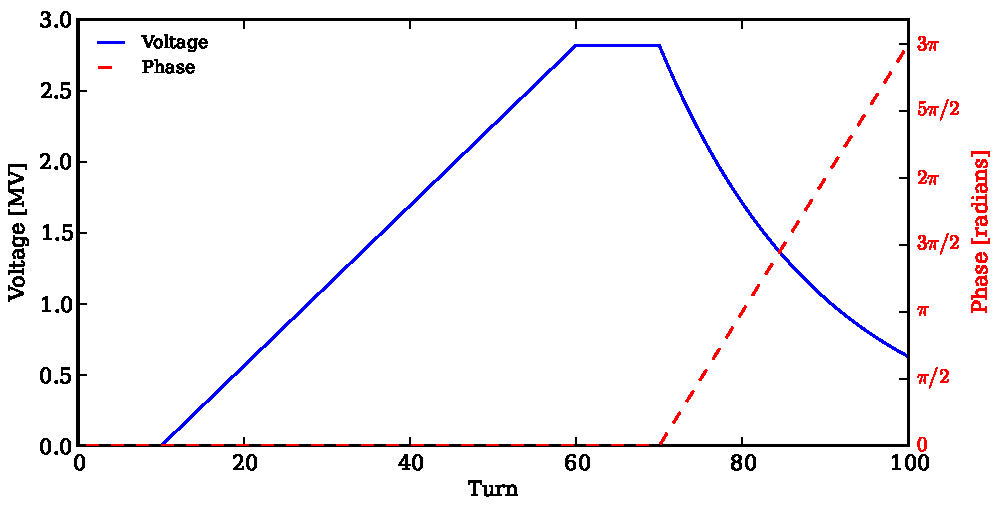
\includegraphics{figures/fail_voltagePhase2v2}
  \caption{Singals generate by \texttt{DYNK} example for ramp + exponential decay of crab voltage, and also linear drift of crab phase. Only the signals for CRAB\_IP1\_L1 are shown. The plot is made from the data in \texttt{dynksets.dat}.}
  \label{fig:DYNK_fail}
\end{figure}

This slightly more complicated example builds on the example given above.
It shows how to change two parameters (voltage and phase) of several objects.
It also demonstrates how functions can be chained together, making more complicated functions.
Some of the resulting functions are shown in Figure~\ref{fig:DYNK_fail}, and the DYNK block here looks like:
\begin{cverbatim}
DYNK
/DEBUG
FUN zero CONST 0.0
FUN CV_R1 GET CRAB_IP1_R1 voltage
FUN CV_R2 GET CRAB_IP1_R2 voltage
FUN CV_R3 GET CRAB_IP1_R3 voltage
FUN CV_R4 GET CRAB_IP1_R4 voltage
FUN CV_L  GET CRAB_IP1_L1 voltage
FUN ramp LIN 0.02 0
FUN ramp_R1 MUL CV_R1 ramp
FUN ramp_R2 MUL CV_R2 ramp
FUN ramp_R3 MUL CV_R3 ramp
FUN ramp_R4 MUL CV_R4 ramp
FUN ramp_L  MUL CV_L  ramp
SET CRAB_IP1_R1 voltage zero 1 10 0
SET CRAB_IP1_R2 voltage zero 1 10 0
SET CRAB_IP1_R3 voltage zero 1 10 0
SET CRAB_IP1_R4 voltage zero 1 10 0
SET CRAB_IP1_L1 voltage zero 1 9 0
SET CRAB_IP1_L2 voltage zero 1 9 0
SET CRAB_IP1_L3 voltage zero 1 9 0
SET CRAB_IP1_L4 voltage zero 1 9 0
/
SET CRAB_IP1_R1 voltage ramp_R1 11 61 -11
SET CRAB_IP1_R2 voltage ramp_R2 11 61 -11
SET CRAB_IP1_R3 voltage ramp_R3 11 61 -11
SET CRAB_IP1_R4 voltage ramp_R4 11 61 -11
SET CRAB_IP1_L1 voltage ramp_L 10 60 -10
SET CRAB_IP1_L2 voltage ramp_L 10 60 -10
SET CRAB_IP1_L3 voltage ramp_L 10 60 -10
SET CRAB_IP1_L4 voltage ramp_L 10 60 -10
/
/Voltage decay and detuning
FUN expCore LIN -0.05 0.0
FUN decay EXP expCore
FUN decayScaled MUL decay CV_L
SET CRAB_IP1_L1 voltage decayScaled 70 100 -70
SET CRAB_IP1_L2 voltage decayScaled 70 100 -70
SET CRAB_IP1_L3 voltage decayScaled 70 100 -70
SET CRAB_IP1_L4 voltage decayScaled 70 100 -70
FUN phasedrift LIN 0.3141592654 0.0
SET CRAB_IP1_L1 phase phasedrift 70 100 -70
SET CRAB_IP1_L2 phase phasedrift 70 100 -70
SET CRAB_IP1_L3 phase phasedrift 70 100 -70
SET CRAB_IP1_L4 phase phasedrift 70 100 -70
NEXT
\end{cverbatim}
The first functions defined here are the same as above, storing the default values (as defined in the single element list) for the relevant elements and also zero.
Then follows a normalized linear ramp function ``ramp'', with gradient $0.02 = 1/50$.
This is then used by the ``specialized'' ramp functions ``ramp\_R1$\cdots$R4'', which scales ``ramp'' so that the end point is the standard voltages for $t\in 0\ldots50$.

These functions are used to first set the crabs to $0.0$ for the first $9$ revolutions, and in the 10th revolution the ramp starts.
As the ``ramp'' function is defined starting at turn $0$, a shift $-10$ or $-11$ is applied to the ramps.
The ramp is switched off after turn 60/61, leaving the crabs to be operating at the last \texttt{SET} value.

Further, we want to demonstrate a failure in the crab voltage.
This is done using an exponential decaying function $V(t) = V_0 \exp\left(-0.05 t\right)$, which is implemented as three chained functions:

\bigskip
\begin{tabular}{@{}lp{0.8\linewidth}}
    \textbf{expCore}     & $f(t) = -0.05 t + 0.0$ \\
    \textbf{decay}       & $g(t) = \exp(f(t)) = \exp(-0.05 t + 0.0)$ \\
    \textbf{decayScaled} & $h(t) = V_0 \cdot g(f(t)) = V_0 \cdot \exp(f(t)) = \exp(-0.05 t + 0.0)$
\end{tabular}

\bigskip
For the \texttt{SET}, the time $t$ is then shifted by $-70$ turns, so that the functions are evaluated starting at $t=0$.

\paragraph{Detuning a cavity (accelerating or crab)}~\\
\todo[inline]{Write}

\paragraph{Using the PIPE function}~\\
%Note: This example is referenced from the FUN table.

To use the \texttt{PIPE} functionality, add a \texttt{FUN} and \texttt{SET} to the \texttt{DYNK} block such as:
\begin{cverbatim}
FUN pipe1 PIPE /tmp/pip1 /tmp/pip2 myID1 4242
SET  ACFCA.AR1.B1 voltage pipe1 10 -1 -9
\end{cverbatim}
Then create the two pipes using the \texttt{mkfifo} UNIX command, e.g.\ \texttt{mkfifo~pip1} and \texttt{mkfifo~pip2} in the chosen directory.
When starting SixTrack, it will first open the input pipe (while reading the DYNK block), and wait for the external program to do the same.
This can be simulated by running \texttt{cat~>~pip1}; it is also possible to open the input pipe before starting SixTrack.
After opening the input pipe, SixTrack will open the output pipe, again this can be simulated by running \texttt{cat~pip2}, and again this pipe may be opened before starting SixTrack.
Note that when SixTrack ends, the output pipe will be closed, so the recieving \texttt{cat} process is terminated.

After opening the output pipe, SixTrack writes the line \texttt{DYNKPIPE~!******************!} to this file.
It then writes a line similar to \texttt{INIT~ID=myID1~for~FUN=pipe1} for each FUN using this output pipe.

During tracking, when one of the \texttt{PIPE} \texttt{FUN}s are called SixTrack writes a line similar to \texttt{GET ID=myID1 TURN=~1} to the output pipe.
Note that the turn number is the one passed to the \texttt{FUN} from \texttt{SET}, i.e. including any turn-shift.
It then waits for a single floating point number to be written (in ascii) to the input pipe, which is then read and returned from the \texttt{FUN}.

% ================================================================================================================================ %
\section{Beam--Beam Element} \label{BeamBeam}

The beam--beam kick, including a separation of the beams, is treated \`{a} la Basetti and Erskine~\cite{BasErs} and implemented as in MAD~\cite{MAD}.
However, a much faster but nevertheless precise calculation using interpolation can be used~\cite{ERIC}.
Since SixTrack version 3, the beam--beam is also available in the 6D form \`{a} la Hirata~\cite{Hirata}.
Lastly, the linear coupling has been considered in 4 and 6 dimensional phase space~\cite{ripbeam}. 

\bigskip
\begin{tabular}{@{}lp{0.8\linewidth}}
    \textbf{Keyword}    & \texttt{BEAM} \\
    \textbf{Data lines} & $>1$ \\
    \textbf{Format}     & Two different input formats are available, ``traditional'' and ``EXPERT''. If ``EXPERT'' mode is wanted, this is triggered by adding the flag \texttt{EXPERT} on the first line of the block.
\end{tabular}

\paragraph{Traditional format}~\\

\bigskip
\begin{tabular}{@{}lp{0.8\linewidth}}
    First line:    & \texttt{partnum emitnx emitny sigz sige ibeco ibtyp lhc ibbc} \\
    Further lines: & \texttt{name ibsix xang xplane xstr}
\end{tabular}

\bigskip
\begin{tabular}{@{}llp{0.65\linewidth}}
    \texttt{partnum}       & float   & Number of particles in bunch \\
    \texttt{emitnx,emitny} & floats  & Horizontal and vertical normalized emittance respectively [$\mu \mbox{m}\cdot\mbox{rad}$] \\
    \texttt{sigz,sige}     & floats  & r.m.s. bunch length [m] and r.m.s. energy spread \\
    \texttt{ibeco}         & integer & Switch (0 = off; 1 = on) to subtract the closed orbit introduced by the separation of the beams. It is recommended to always subtract it as it is not yet calculated in a selfconsistent manner. The \texttt{ibeco} switch also acts on the ``wire'' elements \ref{sec:WIRE} in the same way as on the beam-beam elements. It subtracts the closed orbit introduced by the wire if \texttt{ibeco}=1 and applies it if \texttt{ibeco}=0. \\
    \texttt{ibtyp}         & integer & Switch (0 = off; 1 = on) to use the fast beam--beam algorithms developed in collaboration with G.A.~Erskine and E.~McIntosh.  The linear optics are calculated with ``exact'' beam--beam kicks. \\
    \texttt{lhc}           & integer & For the LHC with its anti--symmetric IR the separation of the beams in one plane can be calculated by the $\beta$--function of the other plane. For flat beams (not anti-symmetric optics) the separation can be loaded from the \texttt{fort.2} file. (0 = off; 1 = anti-symmetric; 2 = load from file). \\
    \texttt{ibbc}          & integer & Linear coupling considered in 4D and 6D (0 = off; 1 = on). \\
    \texttt{name}          &           & Name of 6D beam--beam element. Beam--beam elements that do not appear will be treated as 4D kicks. \\
    \texttt{ibsix}         & integer & Number of slices of the 6D beam--beam element. If \texttt{ibsix} is set to 0 this element is treated as a 4D element. \\
    \texttt{xang}          & float   & Half crossing angle (angle the between the trajectories of the two beams) at this particular element [rad]. \\
    \texttt{xplane}        & float   & Crossing plane angle [rad]. \\
    \texttt{xstr}          & float   & Angle of the position of the slices in the boosted frame [rad] (i.e. $X = Z \sin(\mathit{xstr}) \cos(\mathit{xplane})$, $Y =Z \sin(\mathit{xstr}) \cos(\mathit{xplane})$ ).  In absence of crabbing user should make sure \texttt{xstr=xang}; in case the \texttt{xstr} flag is not set then \texttt{xstr=xang} is assumed and a warning is printed (since version 4.5.45).
\end{tabular}

\paragraph{EXPERT format}~\\

\bigskip
\begin{tabular}{@{}lp{0.8\linewidth}}
    First line:   & \texttt{EXPERT} \\
    Second line:  & \texttt{partnum emitnx emitny sigz sige ibeco ibtyp lhc ibbc} \\
    Further lines & 4D BB lens (1 line per element): \\
                  & ~~~~\texttt{name ibsix $\Sigma_{x,x}$ $\Sigma_{y,y}$ h-sep v-sep strength-ratio} \\
                  & 6D BB lens (3 lines per element): \\
                  & ~~~~\texttt{name ibsix xang xplane h-sep v-sep} \\
                  & ~~~~\texttt{$\Sigma_{x,x}$ $\Sigma_{x,xp}$ $\Sigma_{xp,xp}$ $\Sigma_{y,y}$ $\Sigma_{y,yp}$} \\
                  & ~~~~\texttt{$\Sigma_{yp,yp}$ $\Sigma_{x,y}$ $\Sigma_{x,py}$ $\Sigma_{xp,y}$ $\Sigma_{xp,yp}$ strength-ratio}
\end{tabular}

\bigskip
Some parameters are new or defined in a different way:

\bigskip
\begin{tabular}{@{}llp{0.65\linewidth}}
    \texttt{lhc}   & integer & This parameter is kept for now only for RHIC studies when equal to 9. \\
    \texttt{name}  &         & Name of the beam--beam element. \\
    \texttt{ibsix} & integer & Number of slices of the 6D beam--beam element.\\
                   &         & If \texttt{ibsix} is set to 0, this element is treated as a 4D element.\\
                   &         & If \texttt{ibsix} is larger or equal 1, this element is treated as a 6D element. \\
    $\Sigma_{xx}$  & float   & Horizontal $\sigma$ for the strong beam $\rm{[mm^2]}$. \\
    $\Sigma_{yy}$  & float   & Vorizontal $\sigma$ for the strong beam $\rm{[mm^2]}$. \\
    \texttt{h-sep} & float   & Horizontal beam--beam separation [mm] \\
    \texttt{v-sep} & float   & Vertical beam--beam separation [mm] \\
    \texttt{strength-ratio} & float & Strength ratio with respect to the nominal beam--beam kick strength. This is useful to allow for splitting one beam--beam kick into several (longitudinally close by) kicks.\\
    $\Sigma_{i,j}$ & float   & Second order momenta matrix for the strong beam, in units of mm and mrad. For example $\Sigma_{xxp}$ in [mm\ mrad]
\end{tabular}

\paragraph{Conversion from traditional to EXPERT format}~\\

An automatic converter from the ``traditional'' input block to the new ``expert'' format is built into SixTrack; every time a non-EXPERT input block is encountered, a conversion is printed to the standard output.
Therefore, all the user needs to do is to run SixTrack (number of turns does not matter) on an input file that should be converted, and follow the instructions which are printed at the beginning of the program output.

\paragraph{Remarks:}~\\

These beam--beam elements have to appear in the single element list (~\ref{NonEle}) (type 20).
If the ``traditional'' option is used in the \texttt{BEAM} block, the listing in the single element list must contain their horizontal and vertical beam--beam separations (see~\ref{BBS}).

\paragraph{Sign Convention}~\\

Some clarifications regarding the sign convention used for the separation and crossing angle variables.
%\todo[inline]{Check if applies to both ``traditional'' and ``EXPERT'' format.}

\paragraph{Separations:}~\\
\begin{enumerate}
    \item The separation is added to the transverse coordinates of each particles just before the beam-beam subroutines (see Fig.~\ref{fig:BB_sep}).
        \begin{eqnarray*}
            \tilde x_{i} = x_{i} + \mathrm{sep}_{x} - \mathrm{CO}_{x} \\
            \tilde y_{i} = y_{i} + \mathrm{sep}_{y} - \mathrm{CO}_{y} 
        \end{eqnarray*}
    \item Lorentz boost applied to the updated coordinates.
    \item The separation used for the actual beam-beam kick (sep$_{x,y,kick}$) is the difference between the centroid of the strong slice (X$^{\dag}$,Y$^{\dag}$) and the each particle (x$_i$,y$_i$).
    \item Antiboost to return to accelerator frame.
    \item The separation is removed and the closed orbit is added back. Tracking continues.
        \begin{eqnarray*}
            \tilde x_{i} = x_{i} - \mathrm{sep}_{x} + \mathrm{CO}_{x} \\
            \tilde y_{i} = y_{i} - \mathrm{sep}_{y} + \mathrm{CO}_{y}
        \end{eqnarray*}
\end{enumerate}
\begin{figure}[h]
    \begin{center}
    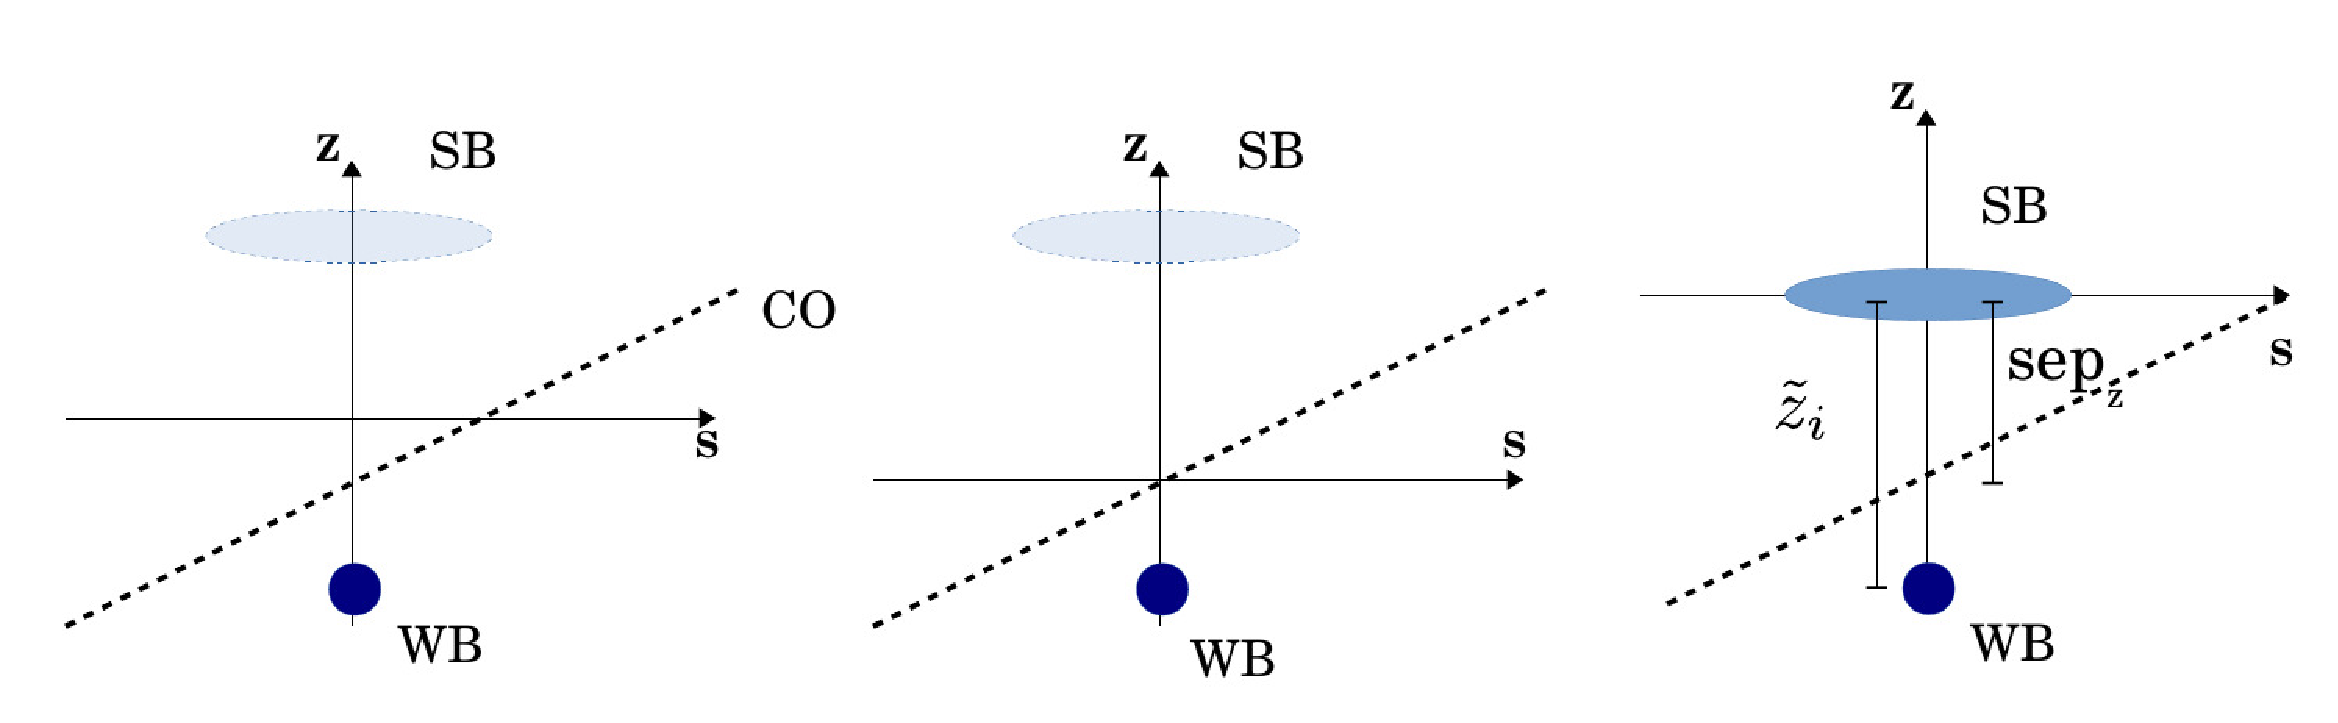
\includegraphics[width=0.8\textwidth]{figures/BB_sep}
    \caption{Coordinate manipulation taking into consideration the beam-beam lens separation as stated in point 1 of the separation sign convention.}
    \label{fig:BB_sep}
    \end{center}
\end{figure}

\paragraph{Crossing angles:}~\\
\begin{enumerate}
    \item The closed orbit is removed just before the beam-beam subroutines.
        \begin{eqnarray*}
            \tilde x^{\prime}_{i} = x^{\prime}_{i} - \mathrm{CO}_{x^{\prime}} \\
            \tilde y^{\prime}_{i} = y^{\prime}_{i} - \mathrm{CO}_{y^{\prime}}
        \end{eqnarray*}
    \item Lorentz boost applied to the updated coordinates.
    \item Apply Synchro-Betatron Mapping.
    \item Antiboost to return to accelerator frame.
    \item The closed orbit is added back. Tracking continues.
        \begin{eqnarray*}
            \tilde x^{\prime}_{i} = x^{\prime}_{i} + \mathrm{CO}_{x^{\prime}} \\
            \tilde y^{\prime}_{i} = y^{\prime}_{i} + \mathrm{CO}_{y^{\prime}}
        \end{eqnarray*}
\end{enumerate}
\begin{figure}[h]
    \begin{center}
    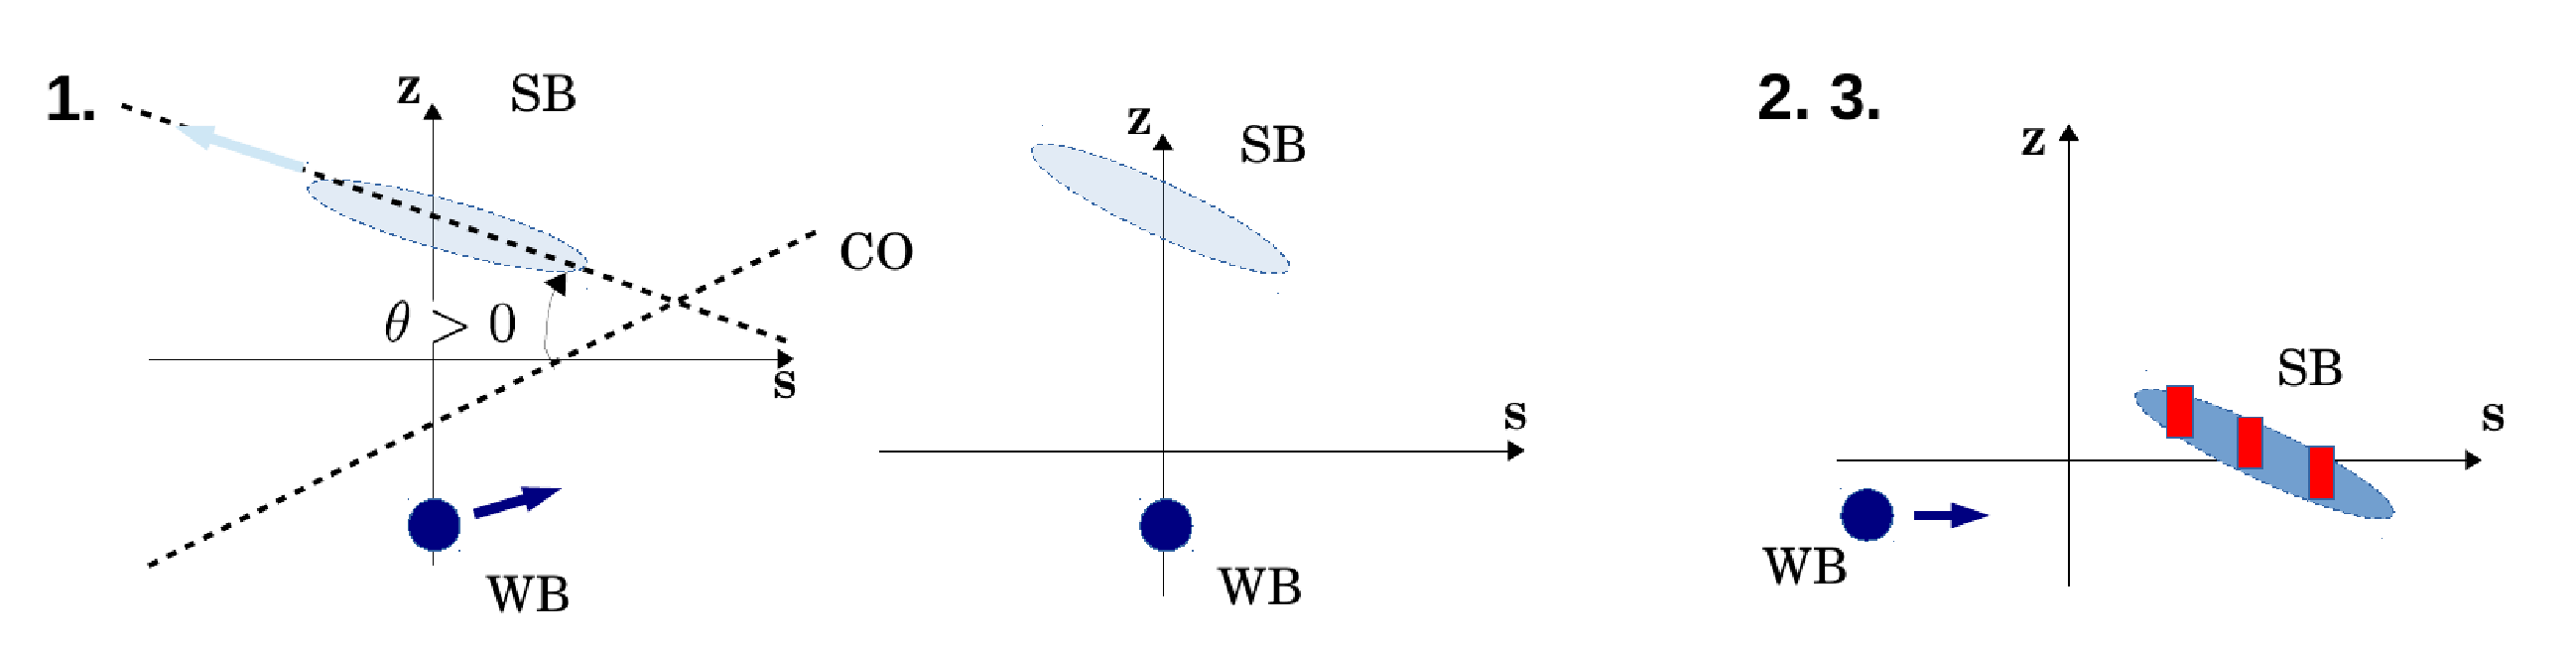
\includegraphics[width=0.8\textwidth]{figures/BB_xsing}
    \caption{Coordinate manipulation to move from the accelerator frame to a head-on collision frame (Figures left and center). A positve crossing angle is considered as shown in the left figure. Then Lorentz boost and Synchro-Betatron Mapping are applied (right).}
    \label{fig:BB_xsing}
    \end{center}
\end{figure}

% ================================================================================================================================ %
\section{Wire} \label{sec:WIRE}

The wire block serves for reading in the input parameters for the wire. Each wire also needs to be added as single element in the list of single elements.

\bigskip
\begin{tabular}{@{}lp{0.8\linewidth}}
    \textbf{Keyword}    & \texttt{WIRE} \\
    \textbf{Data lines} & Variable \\
    \textbf{Format}     & \texttt{name flag\_co current int\_length phys\_length disp\_x disp\_y tilt\_x tilt\_y} \\
                        & A description of the input parameters for the wire is given in Table~\ref{tab:wire}.
\end{tabular}

\begin{center}
\begin{longtable}{|p{2.0cm} |p{1.0cm} |p{9.2cm}|}
    %Note: \\* (with the star) used to inhibit page breaks in the middle of groups of the same type
    \caption{Input parameters for the \texttt{WIRE} block.}
    \label{tab:wire} \\*
    \hline
    \rowcolor{blue!30}
    Arguments & Unit & Description \\*
    \hline
    \endfirsthead

    \hline
    \rowcolor{blue!30}
    Arguments & Unit & Description \\*
    %\hline
    \endhead

    \rowcolor{gray!15}
    \multicolumn{3}{|c|}{(The table continues on the next page)}\\*
    \hline
    \endfoot

    \hline
    \endlastfoot

    \hline

    \texttt{name} & - &
    Name of wire. Must be the same as in list of single elements.\\*
    \hline

    \texttt{flag\_co} & - &
    flag to define the displacement of the wire in respect to the closed orbit or x=y=0. For \texttt{flag\_co}=+1 \texttt{disp\_*} is the distance between x=y=0 and the wire. For \texttt{flag\_co}=-1 \texttt{disp\_*} is the distance between the closed orbit and the wire.\\*
    \hline

    \texttt{current} & A &
    wire current \\*
    \hline

    \texttt{int\_length} & m &
    integrated length of the wire\\*
    \hline

    \texttt{phys\_length} & m &
    physical length of the wire\\*
    \hline

    \texttt{disp\_x} & mm &
    hor. displacement of the wire\\*
    \hline

    \texttt{disp\_y} & mm &
    vert. displacement of the wire\\*
    \hline

    \texttt{tilt\_x} & degrees &
    hor. tilt of the wire $-90 < tilt\_x < 90$ (uses same defintion as DISP block) \\*
    \hline

    \texttt{tilt\_y} & degrees &
    vert. tilt of the wire $-90 < tilt\_y < 90$ (uses same defintion as DISP block) \\*
    \hline		
\end{longtable}
\end{center}

\paragraph{Remarks:}~\\

The user has to check that the wires defined in the WIRE block are also defined in the list of single elements and vice versa.
All parameters, except for the type (type 15), are ignored in the single element definition and the execution is aborted if the parameters are non-zero.
In addition to the parameters defined in the \texttt{WIRE} block, the \texttt{ibeco} parameter in the \texttt{BEAM} block (see Sec.~\ref{BeamBeam}) imposes the same behavior on the wire as for beam-beam.
Explicitly, the closed orbit introduced by the wire is subtracted if \texttt{ibeco}=1 and not subtracted if \texttt{ibeco}=0.

\paragraph{Example:}~\\

In the following we give some examples for wire definitions. This example defines two wires wire\_1 and wire\_2.

The input block in \texttt{fort.3} is given by:
\begin{cverbatim}
WIRE
wire_1   -1  +98.9   2.0  1.0   10.0   10.0     1.1     1.1
wire_2   -1  +98.9   2.0  1.0   10.0   10.0     0.0     0.0
NEXT
\end{cverbatim}
The single and structure element definition in \texttt{fort.2} is given by:
\begin{cverbatim}
SINGLE ELEMENTS---------------------------------------------------------
...
wire_1           15   0.000000000e+00   0.000000000e+00 
0.000000000e+00    0.000000000e+00    0.000000000e+00    0.000000000e+00
wire_2           15   0.000000000e+00   0.000000000e+00 
0.000000000e+00    0.000000000e+00    0.000000000e+00    0.000000000e+00
...
STRUCTURE INPUT---------------------------------------------------------
...
BLOC56            wire_1              wire_2
...
\end{cverbatim}
Note that all parameters except for the type have to be set to 0 in the single element definition.

% ================================================================================================================================ %
\section{``Phase Trombone'' Element} \label{Trombone}

The linear ``phase trombone'' allows the introduction of a change in the transverse phases without spoiling the linear optics of the rest of the machine, i.e. the Twiss parameters are the same at entrance and exit of the element.

\bigskip
\begin{tabular}{@{}lp{0.8\linewidth}}
    \textbf{Keyword}    & \texttt{TROM} \\
    \textbf{Data lines} & 1 line with name and then in blocks of 14 lines with 3 entries each. \\
    \textbf{Format}     & First line: \texttt{name} \\
                        & Second line: \texttt{cx, cx', cy} \\
                        & Third line: \texttt{cy', cz, cz'} \\
                        & Fourth util $15^{th}$: \texttt{M($ 6 \times 6$)} matrix 
\end{tabular}

\bigskip
\begin{tabular}{@{}llp{0.6\linewidth}}
    \texttt{name} & string & May contain up to 47 characters \\
    \texttt{cx, cx', cy, cy', cz, cz'} & floats & 6D closed orbit to be added to the coordinates. \\
    \texttt{M($ 6 \times 6$)} & floats & $ 6 \times 6$ matrix elements
\end{tabular}

\paragraph{Remarks:}~\\

The user has to make sure that the above stated conditions are fulfilled.
When using the $mad\_6t$~\cite{CONVERTOR} converter from MAD-X to SixTrack, this is guaranteed to be the case.
Note also that the crossterms between the transverse plains are not considered for the time being.

% ================================================================================================================================ %
\section{Beam Distribution EXchange (BDEX)} \label{sec:BDEX}

The Beam Distribution EXchange allows an external program to read and modify the beam distribution in SixTrack.
This can be used for tracking part of the machine in an external program, for example for including physics processes that are normally not available in SixTrack.
Another possible use is for multi-bunch tracking, i.e.\ with an external program ``swapping'' the bunch at a some point in the ring.
This would be useful for studying (for example) beam loading, where the external program would read the position of a bunch in the cavity, use that to compute an update of the cavity voltage (which can be sent to SixTrack using DYNK FUN PIPE), swap the bunch with another one and track that to the cavity (still at ``physics turn'' 1, but ``SixTrack turn'' 2) etc.

Please note that \texttt{BDEX} is currently not supported in the checkpoint/restart version or in the collimation version.
Including \texttt{BDEX} in one of these versions results in a run-time error.

\bigskip
\begin{tabular}{@{}lp{0.8\linewidth}}
    \textbf{Keyword}    & \texttt{BDEX} \\
    \textbf{Data lines} & Variable \\
    \textbf{Format}     & There are three types of statements possible in a BDEX block, listed below.
\end{tabular}

\bigskip
Additionally, lines starting with ``/'' are treated as comments and are ignored.

\paragraph{ELEM} \texttt{ELEM chanName elemName action}\\

This associates a given element with an already existing channel and an action.
The element must appear in the SINGLE ELEMENT block, and be of type 0 (marker).
The action indicates what should be done with the particle distribution when it reaches this element.
Currently, the only allowed action is ``1'', which means ``particle exchange'', i.e.\ output the beam distribution and read back another one at the same point.

\paragraph{CHAN} \texttt{CHAN chanName chanType \ldots}\\

This creates a new channel through which the \texttt{BDEX} can communicate.
Currently, the only implemented \texttt{chanType} is \texttt{PIPE}, however \texttt{TCPIP} is also foreseen.

For the \texttt{PIPE} type, the statement including arguments is \texttt{CHAN PIPE inPipeName outPipeName format fileUnit}.
This uses a pair of UNIX FIFOs, through which SixTrack can comunicate with an external program.
When the channel is used, it sends a message on the outpipe, then waits for a reply with the new distribution over the inPipe.
The \texttt{format} is an integer used to indicate the output/input format, and is currently unused.
The \texttt{fileUnit} is the Fortran unit number that should be used to open the inPipe.
The \texttt{outPipe} is opened on the next unit, so both units fileUnit and fileUnit+1 must be free.

\paragraph{DEBU}~\\

This statement switches on extra ``debugging'' output from \texttt{BDEX}.
This can be useful if debugging the code or if debugging the input.

\subsection{Communication protocols}

The communication protocols used by the different channel types are listed below:

\paragraph{PIPE communication protocol}~\\

When a pair of pipes are first initialized, a header ``\texttt{BDEX-PIPE !******************!}'' is written to the output pipe.
Then, when the tracking reaches an element which is marked as active for this channel, it writes another header like ``\texttt{BDEX TURN= 1 BEZ=ip1 I= 1 NAPX= 64}'', where \texttt{TURN} is the number of the current SixTrack turn, \texttt{BEZ} the name of the SINGLE ELEMENT, \texttt{I} the index of the STRUCTURE ELEMENT, and \texttt{NAPX} the number of particles to be written out.
After this follows \texttt{NAPX} lines with the particle information (one per particle), each line of the format \texttt{xv(1,j) yv(1,j) xv(2,j) yv(2,j) sigmv(j) ejv(j) ejfv(j) rvv(j) dpsv(j) oidpsv(j) dpsv1(j),nlostp(j)} where all but the last floating point numbers, the last being an integer.
Finally, it writes ``\texttt{BDEX WAITING...}'' to the output pipe, and waits for data on the input pipe.

The first line expected on the input pipe should be an integer containing the number of particles to write back.
If this integer is -1, the current particle distribution is kept.
Otherwise, a number of lines of the same format as with the output is expected.
After reading in the expected number of particles, the string ``\texttt{BDEX TRACKING...}'' is written to the output pipe and tracking is resumed.

\paragraph{TCPIP communication protocol}~\\

TCPIP is not yet implemented, as it would require an external library.
The FLUKA version implements this, we should make sure that we are compatible with their requirements and ideally their protocol.

\paragraph{Example}~\\

\todo[inline]{Example BDEX block, example manual usage, example minimal Python program (location or listing).}

% ================================================================================================================================ %
\section{Electron lens} \label{sec:elen}

The electron lens module serves for reading in the input parameters for different types of electron lenses.
Each e-lens also needs to be added as single element in the list of single elements.
Currently the ideal electron lens is implemented, i.e.~with no errors in the e-beam distribution.

\bigskip
\begin{tabular}{@{}lp{0.8\linewidth}}
    \textbf{Keyword}    & \texttt{ELEN} \\
    \textbf{Data lines} & Variable \\
    \textbf{Format}     & \texttt{name type theta\_r2 r2 r1 offset\_x offset\_y flag\_entrance flag\_exit $\sigma$} \\
                        & A description of the input parameters for the different e-lens types is given in Table~\ref{tab:elen}. Currently the ideal electron lens is implemented in SixTrack, i.e.~with no errors in the e-beam distribution.
\end{tabular}

\begin{center}
\begin{longtable}{|p{2.0cm} | p{2.4cm} p{1.0cm} p{9.0cm}|}
    %Note: \\* (with the star) used to inhibit page breaks in the middle of groups of the same type
    \caption{Input parameters for \texttt{ELEN} block.}
    \label{tab:elen} \\*
    \hline
    \rowcolor{blue!30}
    Type Name & Arguments & Unit & Description \\*
    \hline
    \endfirsthead

    \hline
    \rowcolor{blue!30}
    Type Name & Arguments & Unit & Description \\*
    %\hline
    \endhead

    \rowcolor{gray!15}
    \multicolumn{4}{|c|}{(The table continues on the next page)}\\*
    \hline
    \endfoot

    \hline
    \endlastfoot

    \hline
    \rowcolor{blue!15}
    \multicolumn{4}{|l|}{Valid for all types} \\*

    & \texttt{name} & -- & Name of e-lens. Must be the same as in list of single elements.\\*
    \hline

    & \texttt{type} & -- & Type of e-lens. Available types are \texttt{UNIFORM} and \texttt{GAUSSIAN}. \\*
    \hline

    & \texttt{theta\_r2} & mrad & Kick received at $r=r_2$ where $r_2$ is the outer radius of the electron lens.\\*
    \hline
    
    & \texttt{r2} & mm & Outer radius of e-lens.\\*
    \hline
    
    & \texttt{r1} & mm & Inner radius of the e-lens. Can be 0 but not negative.\\*
    \hline
    
    & \texttt{offset\_x} & mm & Horizontal offset of e-lens.\\*
    \hline
    
    & \texttt{offset\_y} & mm & Vertical offset of e-lens.\\*
    \hline
    
    & \texttt{flag\_entrance} & -- & Enable bends at entrance of e-lens (not yet implemented).\\*
    \hline
    
    & \texttt{flag\_exit} & -- & Wnable bends at exit of e-lens (not yet implemented).\\*
    \hline
    
    \rowcolor{blue!15}
    \multicolumn{4}{|l|}{Type specific parameters} \\*
    
    \texttt{GAUSSIAN} & \texttt{$\sigma$} & mm & Sigma of the e-beam.\\*
\end{longtable}
\end{center}

\noindent Currently, two types of electron beam profiles are supported:

\bigskip
\begin{tabular}{@{}llp{0.6\linewidth}}
    \texttt{UNIFORM}  & e-beam with constant density of electrons. \\
    \texttt{GAUSSIAN} & e-beam with a radial Gaussian profile. \\
\end{tabular}

The spacial charge density of all profiles is defined between \emph{r1} and \emph{r2}:
\begin{equation}
  \rho(r)=\left\{
    \begin{array}{ll}
        0 & \mbox{if $r \le r_1$} \\
        f(r) & \mbox{if $r_1 < r < r_2$} \\
        0 & \mbox{if $r_2 \le r$} \\
    \end{array}
    \right. \\
\end{equation}
Moreover, if $r_1=0$, then the lens is full; otherwise, it is hollow.

\paragraph{Remarks:}~\\

The user has to check that the e-lens defined in the \texttt{ELEN} block is also defined in the list of single elements and vice versa.
All parameters except for the type (type 29) are ignored in the single element definition.
The implementation of the \texttt{UNIFORM} and \texttt{GAUSSIAN} types (ideal e-lenses) has no explicit energy-dependency, except for the user defined parameter \texttt{theta\_r2} (see \cite{sixphys}).

\paragraph{Examples:}~\\

In the following we give some examples for e-lens definitions.
The example defines two electron lenses hel1 and hel2.
The former is a hollow e-lens, with a uniform electron density for cleaning purposes; the latter has a Gaussian electron beam profile.
The input block in \texttt{fort.3} is then given by:
\begin{cverbatim}
ELEN
hel1 UNIFORM 4.920e-03 6.928 4.619 1.1547 2.3093 0 0
hel2 GAUSSIAN 4.920e-03 6.928 4.619 1.1547 2.3093 0 0 0.3
NEXT
\end{cverbatim}
The single and structure element definition in \texttt{fort.2} is given by:
\begin{cverbatim}
SINGLE ELEMENTS---------------------------------------------------------
...
hel1            29   0.000000000e+00   0.000000000e+00 
   0.000000000e+00    0.000000000e+00    0.000000000e+00    0.000000000e+00
hel2            29   0.000000000e+00   0.000000000e+00   
   0.000000000e+00    0.000000000e+00    0.000000000e+00    0.000000000e+00
...
STRUCTURE INPUT---------------------------------------------------------
...
BLOC56            hel1              hel2
...
\end{cverbatim}
Note that all parameters except for the type are set to 0 in the single element definition.

% ================================================================================================================================ %
\section{Scattering} \label{sec:scatter}

{\color{notered}\textbf{Note: }This module is experimental! Use at your own risk; both the input format and physics implementation may change.}

\bigskip
The \texttt{SCATTER} module is a framework for scattering particles through Monte Carlo processes at various points in the machine.

\bigskip
\begin{tabular}{@{}lp{0.8\linewidth}}
    \textbf{Keyword}    & \texttt{SCAT(TER)} \\
    \textbf{Data lines} & Variable \\
    \textbf{Format}     & There are several different main statement classes possible in a \texttt{SCATTER} block, listed below.
\end{tabular}

\bigskip
Lines starting with ``/'' are treated as a comment and ignored

\paragraph{DEBUG} \texttt{DEBUG}\\

This statement switches on extra ``debugging'' output from \texttt{SCATTER}.
This can be useful if debugging the code or if debugging the input.

\paragraph{ELEMent} \texttt{ELEM elemname profile scaling gen1 (gen2, (gen3))}\\

This statements associates a \texttt{PRO}file and between one and 3\footnote{Controlled by the parameter \texttt{scatter\_maxGenELEM}.} \texttt{GEN}erators with a SINGLE ELEMENT which must be of type 40, as described in Section~\ref{SCAT}.
The \texttt{scaling} argument, which is a floating point number, is used to scale the probability of an interaction.
This can be controlled through DYNK, for example in order to scale only at one specified turn.
The \texttt{PRO}file, \texttt{GEN}erator(s), and single elements are referenced through their names, and for the \texttt{GEN}erators and \texttt{PRO}file they must be defined above the \texttt{ELEM}ent in the \texttt{SCATTER} block.

\paragraph{PROfile} \texttt{PRO name type (arguments)} \\

This statement defines a profile, that is a density profile and general properties of the targets which with the tracked particles are colliding.
Several different types are available:

\bigskip
\noindent\texttt{PRO name FLAT density[targets/cm$^2$] mass[MeV/c$^2$] momentum[MeV/c]}\\

\bigskip
\noindent\texttt{PRO name GAUSS1 beamtot[particles] sigmaX[mm] sigmaY[mm] offsetX[mm] offsetY[mm]} \\

The \texttt{GAUSS1} profile type us given by
\begin{align}
    \rho(x,y) = \frac{N_{\mathrm{tot}}}{2\pi\sigma_x\sigma_y}
                \exp\left(-\frac{(x-\mu_x)^2}{2\sigma_x^2}\right)
                \exp\left(-\frac{(y-\mu_y)^2}{2\sigma_y^2}\right).
\end{align}

\paragraph{GENerator} \texttt{GEN name type (arguments)} \\

The generator block takes a name and a generator type input, followed by the parameters for the
generator type.

\bigskip
\noindent\texttt{GEN name PPBEAMELASTIC a b1 b2 phi tmin (crossSection)} \\

Takes five or six input arguments, and generates the probability distribution given by
\begin{align}
    g(t) = \frac{1}{a_1^2}\frac{d\sigma}{dt} = e^{-b_1 t}+ 2ae^{-(b_1+b_2)t/2}\cos{\phi} + a^2e^{-b_2 t},
\end{align}
where the first expression is a soft scatter data fit, the third expression a hard scatter fit, and the second expression is the interference. $a = a_2/a_1$ is the amplitudes of the expressions. These are combined into the first four input arguments $a$, $b_1$, $b_2$, and $\phi$, as well as $t_{min}$ which provides a cut-off limit.
The optional sixth argument defines a fixed cross section for the scattering probability.

Input example with values for a fit to 13 TeV LHC.
\begin{cverbatim}
GEN  sc_thin     PPBEAMELASTIC 0.046 18.52 4.601 2.647 0.0 30e-27
\end{cverbatim}

\paragraph{SEED} \texttt{SEED seed1 seed2}\\

This sets the seed of the internal RNG used by the SCATTER block \todo{Cite RANECU}.
Two integer seeds are required, for this block.
The \texttt{SEED} block is mandatory for the SCATTER block to work.
Note that when running several simulations, the seed settings must be varied between each run in order to get uncorrelated results.
